\section{State of the Art }
def: State of the art
\textit{ State of the art is the level of knowledge and development achieved in a technique,science, etc, esp at present }
\newline
This section will be an analysis of a number of applications that all focus on designing a room or a set of rooms. The previous sections have provided the necessary framework for doing the analysis. specifically the analysis will cover:

\begin{itemize}
\item the familiarity the of the different aspects of the apps.\\
what parts of the app have been seen in other apps or in real life. 
\item the knowledge space for the app\\
here the analysis will try to determine if the app succesfully bridges the knowledge gap talked about in ux section ref: fig. \ref{fig:Knowledge}.
\item The graphical design: Color, overall layout. Farver, fonts og sådan overall lauout
\item the different interaction methods that is used. 
\end{itemize}
 finally the end of this section will sum up the trends noted and will give a overview of what aspects the different applications have lacked behind with and what aspects this project could aim to improve. 

\subsection{Ikea Kitchen Planner}
In this application customers can create accurate measurements of their own kitchen and place the furniture from IKEAs catalogue. It is possible to do different wall measurements, add wallpapers to walls, apply different ceiling and floor covers, add windows and doors. Users can view the layout from top-down view and later see how furnitured layouts look in 3D perspective.

IKEA’s web application for designing kitchens is used mainly in actual IKEA stores.This could indicate that users need help using this application It is used as a tool with focus on efficiency and not so much an app you would use at home for interior design. Most of the people that were asked in the initial interview also confirmed that they do not use this application. Some of the participants are familiar with the app and have tried the it but do not use it. 

When you first enter the app there are no immediate help or tutorial. There is, however, two places in the app where it is possible to get help yourself. Very reasonable layout going from left to right and top to bottom.  There is a lot of easy-recognizable buttons which helps the user experience along. 
It is very slow though and highly affects the usability. 

\begin{figure}[H]
\centering
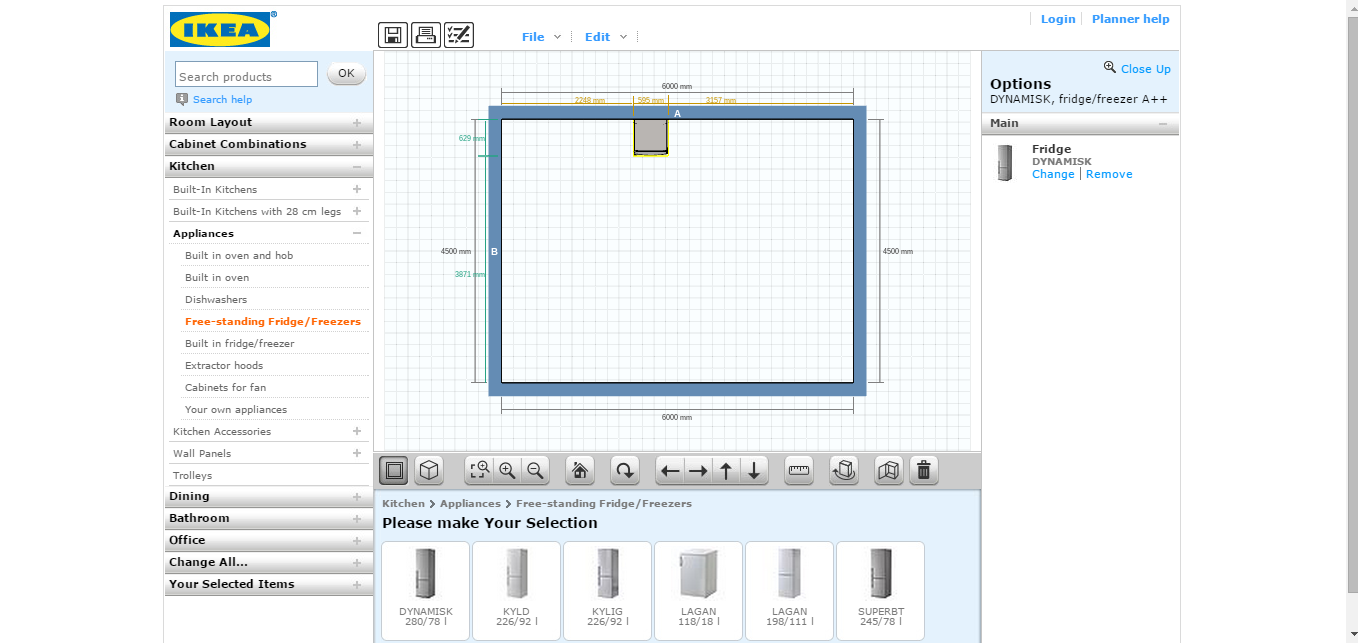
\includegraphics[scale=0.125]{IKEAPlanner.png}
\caption{IKEAs kitchen planner webapplication in 2D mode.}
\end{figure}

The app is grey and clinical but again, it is a practical tool for IKEA customers to visualize a kitchen. 
The application offers plenty of useful features and can be used to give a grasp of how people’s homes would look like prior to buying the actual items, however, it is rarely used by IKEA’s customers. The problem could be that the application is hard to use, leading to long time spans used to build the desired kitchen design. A solution to this possible problem could be to create an application that is more intuitive and takes less time to achieve the user’s needs.

\subsection{HomeDesign3D}
This mobile application is made for interior design. It has most of the basic features; building rooms, placing furniture, windows and doors. The user can then switch to a 3D view. Here there is two settings to choose from - a joystick where you use both thumbs to move around the house, or arrows where you can view the room by moving your finger around and use the arrows to move from room to room. From the 3D view you can paint the walls and change flooring.

\begin{figure}[H]
\centering
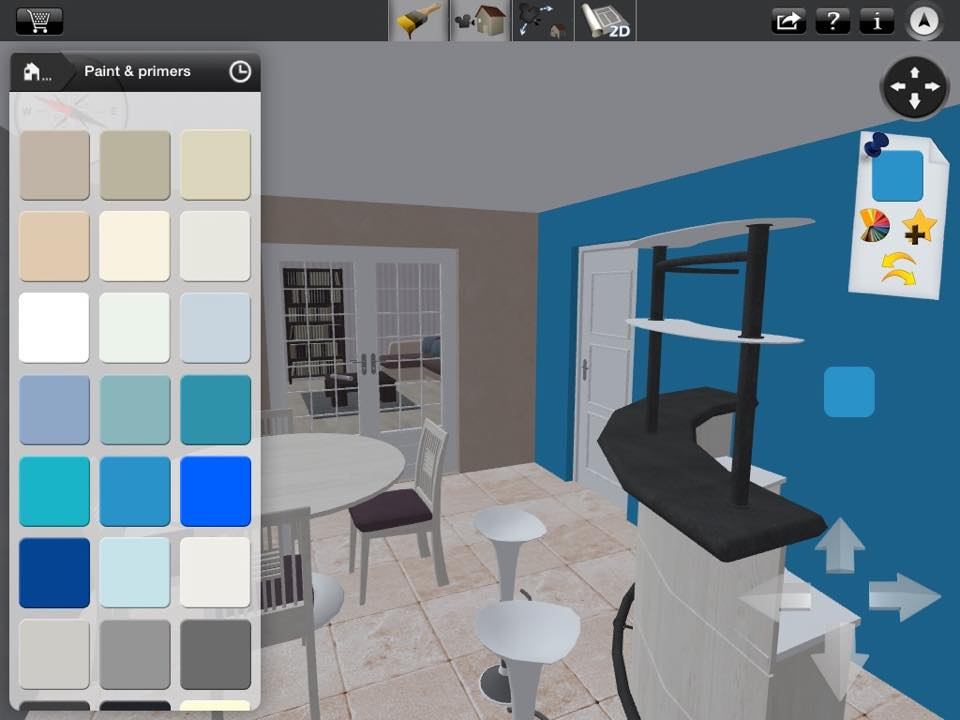
\includegraphics[scale=0.125]{HomeDesign3D.jpg}
\caption{HomeDesign3D application. Painting walls.}
\end{figure}

When you first enter the app you are faced with the option of buying the full version. This is actually the start of a long tutorial. It is very hard to notice though, since the points at the bottom that indicates that you can swipe is overrun by a commercial. It is very unlikely that the user will find this help from the beginning and therefore will properly “go back” to the menu. The tutorial is easy to understand but very long. It has both pictures and text. It looks messy because of the background and the hand drawn hand that shows how to do the different thing. It is not very consistent in matters of graphical design. 
You can find this app later on in the menu. 
The next step is the design. There is apparently no start menu or the likes. 

The icons are easy recognizable.  

The layout looks very cluttered. There is the big commercial at the bottom and the menu bar in the top. 
The mix of the cool black bars and buttons with the beige background does not go very well together. The fact that the background is textured as a wall as well does not help the graphical aspect of this app. 

\subsection{AutoDesks HomeStyler}
This app is autodesks attempt at making an interior design app. the app does not provide a user  guide  from when you open up the app, this is opposed to the idea about bridging the knowledge gap with tutorials. The app does 
however provide a guide for users, once they are actually designing their room, but if the user is not able to get 
to this point then they are stuck. The overall look of the app is reminiscent of the flat design pattern as seen 
in Windows 8, this makes the app feel very modern. it also makes the app look very exclusive. However during the 
main activity of the app the design does not exactly match the look when browsing the catalogue, this leads to the 
app lacking consistency. 

\begin{figure}[H]
\centering
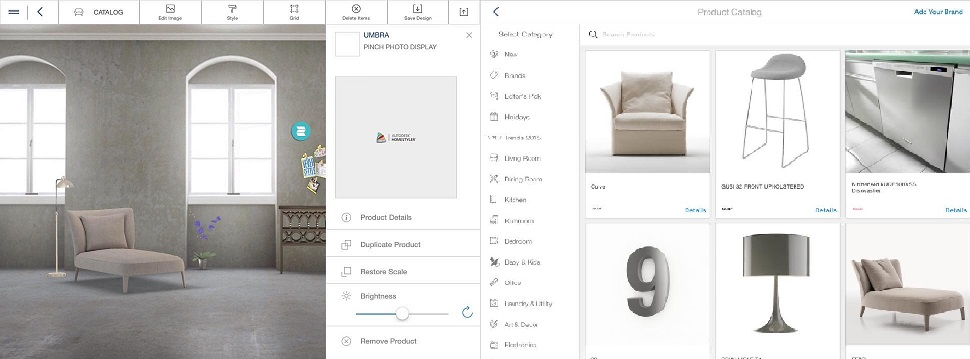
\includegraphics[scale=0.125]{AutodeskCombined.jpg}
\caption{Homestylers lack of consistency. Right: The design of the catalogue. Left: The design of the actual room planning feature.}
\end{figure}

The app’s button design also seem to be focused on bigger screens than a smartphone. The 
big button at the top, labeled “Redesign” is a good example of both the isolation effect mentioned in \ref{idas 
section}\todo{fix reference to reference to Idas section on the isolation effect} and also the button follows the principle of having the buttons be labeled with a single word 
\ref{robinsonUX}. the interaction in the app is primarily clicks, with some multi touch functions for the more 
advanced functions such as resizing, moving, rotating furniture, these functions are explained the first time the 
user is using them and then never again.

\subsection{Planner5D}

Planner5D is an application made both for web and mobile. The web is however better executed than the mobile version. This app allows you to build rooms and place furniture, windows etc. 

\begin{figure}[H]
\centering
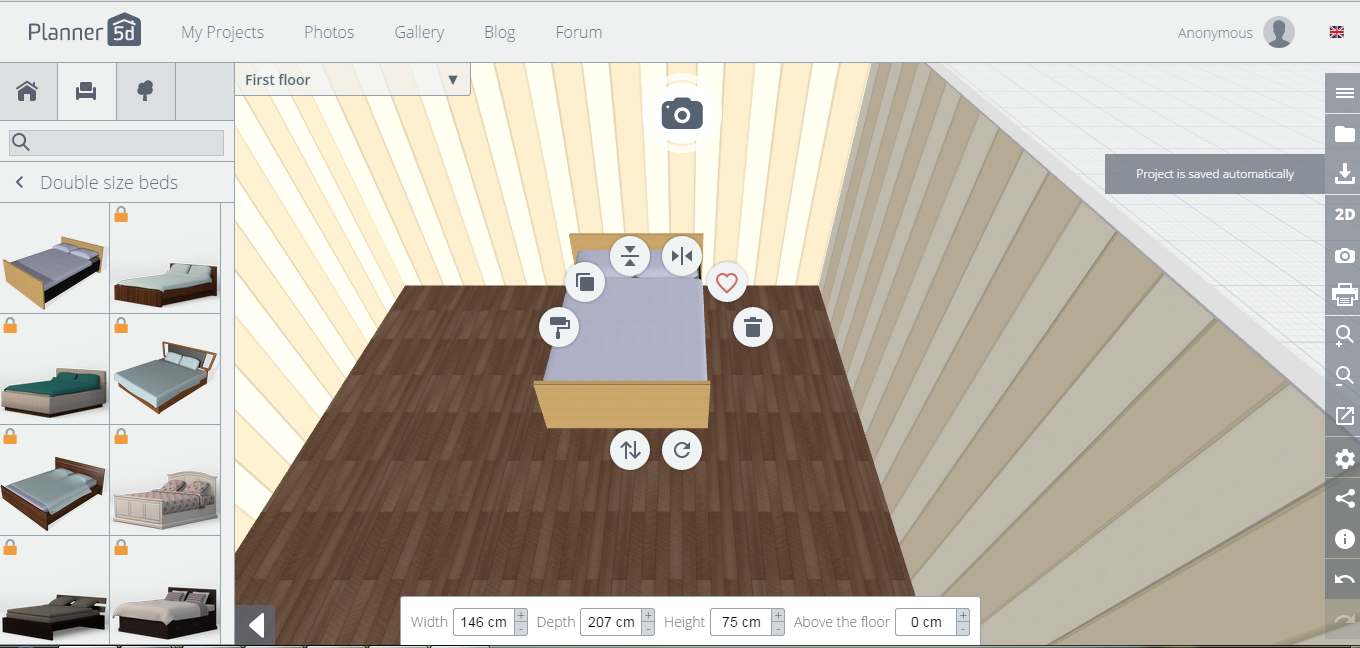
\includegraphics[scale=0.125]{Planner5D.png}
\caption{Planner5D, placing furniture.}
\end{figure}

Start screen gives nice tutorials but are primarily composed of text. The knowledge gap is very tiny, close to nothing.
The menu bars are well divided into four sections.
The menu on the left is very apple like in its graphical feedback. Besides this there is a toolbox which is nicely divided by category, a bar at the top for social/profile aspects and lastly a menu that appears when you have placed a piece of furniture in the room; this is only in icons and no text hovers over this which makes it unclear what the different buttons do since the icons are not very familiar. A lot of focus on user friendliness. 

The app uses mainly point and click with drag.

The graphic design is very minimalistic and modern. The different features has been nicely placed which puts the focus on your own design. 

Furniture interaction does not match the real life movements of the user.

\subsection{Conclusion}



\section{Design Requirements}

\begin{itemize}
\item familiarity
\item non-traditional interaction explained without text
\item uphold one of the two conditions from the knowledge gap bit. 
\item make UI elements obvious(make use of isolation)
\item collapsible umbrella style UI
\item make use of accelerometer/gyroscope
\item stick to one color scheme
\item limit amount of information given to the user
\end{itemize}
